\documentclass[11pt,a4paper]{article}

% --- packages -------------------------------------------------------------
\usepackage[utf8]{inputenc}
\usepackage[T1]{fontenc}
\usepackage[margin=1in]{geometry}
\usepackage{amsmath,amssymb}
\usepackage{graphicx}
\usepackage{booktabs}
\usepackage{array}
\usepackage{longtable}
\usepackage{xcolor}
\usepackage{listings}
\usepackage{caption}
\usepackage[hidelinks]{hyperref}

% --- listings style -------------------------------------------------------
\definecolor{codegray}{gray}{0.95}
\lstset{
  basicstyle=\ttfamily\footnotesize,
  backgroundcolor=\color{codegray},
  breaklines=true,
  frame=single,
  language=Python,
  keywordstyle=\color{blue!60!black},
  commentstyle=\color{green!40!black},
  stringstyle=\color{red!60!black},
  showstringspaces=false,
}

\newcommand{\ee}[1]{\times 10^{#1}}
\newcommand{\code}[1]{\texttt{#1}}

% --- title ----------------------------------------------------------------
\title{\bfseries FET Biosensor Device Simulation with the DDM.SPC Solver\\[4pt]
\large Theory, Physics and Implementation of Four ISFET/BioFET Models}
\author{Computational Device \& Electrochemistry Study\\
\small Generated for the \code{CODEC-26} repository}
\date{\today}

\begin{document}
\maketitle

\begin{abstract}
\noindent
This document gives the physical and mathematical background for four
Python programs that model \emph{ion-sensitive} and \emph{biologically-sensitive
field-effect transistors} (ISFET/BioFET) --- the dominant electronic transducers
for label-free disease detection --- built on the two-dimensional
drift-diffusion + Schr\"odinger--Poisson device solver \textbf{DDM.SPC}. The four
programs form a fidelity ladder: (i)~\code{biosensor\_isfet.py}, a MOS-capacitor
front-end; (ii)~\code{biosensor\_isfet\_transfer.py}, a full-device
drain-current transfer-curve model; (iii)~\code{double\_layer.py}, a
self-consistent electrolyte site-binding + Gouy--Chapman--Stern double-layer
module; and (iv)~\code{biosensor\_isfet\_gdl.py}, which couples the electrolyte
module to the device solver to produce a physically realistic, \emph{sub-Nernstian}
biosensor. Rather than repeat every topic for every file, we present the shared
device physics once, the electrolyte physics once, and then a tabular comparison
that maps each program onto the theory, together with the simulated results and
their application to disease detection.
\end{abstract}

\tableofcontents

% =========================================================================
\section{Introduction and background}
\label{sec:intro}

\subsection{Field-effect biosensors}
An ISFET, introduced by Bergveld in 1970, is a MOSFET whose metal gate is
replaced by an electrolyte contacted through a reference electrode and a
chemically sensitive insulator surface \cite{bergveld1970,bergveld2003}. The
quantity being sensed --- proton activity (pH), a specific ion, or the charge of
a captured biomolecule (DNA strand, antigen, enzyme product) --- modifies the
electrostatic potential at the insulator/electrolyte interface. That interfacial
potential adds directly to the effective gate bias, shifting the transistor
threshold voltage $V_{\mathrm{th}}$ and hence the drain current. Because the
readout is a purely electrical, label-free threshold shift, field-effect
biosensors underpin point-of-care diagnostics: pH and metabolic panels, DNA-FET
pathogen detection, ImmunoFET antigen assays (troponin, C-reactive protein), and
enzymatic glucose sensing \cite{poghossian2014,schoning2002}.

\subsection{The DDM.SPC solver}
DDM.SPC (\emph{Drift-Diffusion Model + Schr\"odinger--Poisson Correction}) is a
general-purpose 2-D, steady-state, finite-element semiconductor device solver.
It solves the coupled Poisson and electron/hole continuity equations in the
quasi-Fermi-potential formulation with a fully coupled Newton method and the
exact analytic Jacobian, and supports heterojunctions, SRH/Auger/radiative
recombination, Fermi--Dirac statistics, an insulated (MOS) gate referenced to a
metal work function, Schottky contacts, and an optional self-consistent
Schr\"odinger--Poisson quantum-confinement correction. The insulated-gate model
is the key enabler here: the analyte-induced interfacial potential enters exactly
as a shift of the gate work function, so the whole ISFET/BioFET family is
representable with the existing solver.

\subsection{Scope of the four programs}
The four programs progress from an idealised demonstration to a physically
realistic biosensor:
\begin{enumerate}
  \item \textbf{\code{biosensor\_isfet.py}} --- the MOS-capacitor front-end.
  Establishes the transduction principle (analyte $\to$ gate work function $\to$
  surface potential / threshold) with a robust, mesh-free structured solve.
  \item \textbf{\code{biosensor\_isfet\_transfer.py}} --- the complete transistor.
  Computes drain-current transfer curves $I_D(V_G)$ and extracts the three
  figures of merit (threshold shift, sub-threshold swing, sensitivity).
  \item \textbf{\code{double\_layer.py}} --- the electrolyte interface physics
  (site-binding + Gouy--Chapman--Stern) that the device solver lacks; it produces
  the surface potential $\psi_0$ as a function of pH, ionic strength, and bound
  biomolecule charge.
  \item \textbf{\code{biosensor\_isfet\_gdl.py}} --- couples (iii) into the device
  solve so the analyte-to-gate coupling becomes realistically \emph{sub-unity}
  (sub-Nernstian pH response and Debye-limited biomolecule detection).
\end{enumerate}

% =========================================================================
\section{Shared device physics}
\label{sec:device}

All four programs rest on the same semiconductor transport core; we state it once.

\subsection{Drift-diffusion in quasi-Fermi variables}
The primary nodal unknowns are the normalised electrostatic potential
$u=\psi/V_T$ and the electron/hole quasi-Fermi potentials $v=\phi_n/V_T$,
$w=\phi_p/V_T$, where $V_T=k_BT/q$ is the thermal voltage. Carrier densities
follow from Boltzmann statistics,
\begin{equation}
  n = n_i\,e^{\,u-v}, \qquad p = n_i\,e^{\,w-u},
  \label{eq:boltzmann}
\end{equation}
so the law of mass action $np=n_i^2$ holds at equilibrium ($v=w=0$). With the
net scaled doping $C=(N_D-N_A)/n_i$, the three coupled Galerkin weak forms solved
by DDM.SPC are Poisson's equation and the two steady-state continuity equations,
\begin{align}
  \nabla\!\cdot\!(\varepsilon\nabla\psi) &= -q\,(p-n+N_D-N_A), \label{eq:poisson}\\
  \nabla\!\cdot\mathbf{J}_n &= +q\,R, &
  \mathbf{J}_n &= q\mu_n n\nabla\phi_n, \label{eq:jn}\\
  \nabla\!\cdot\mathbf{J}_p &= -q\,R, &
  \mathbf{J}_p &= q\mu_p p\nabla\phi_p, \label{eq:jp}
\end{align}
where $R$ is the net recombination rate (Shockley--Read--Hall + Auger; zero in
the ideal-diffusion limit). Linear-triangle finite elements and 3-point Gauss
quadrature assemble the residual and its analytic $3N\times 3N$ Jacobian, which
is solved by damped Newton iteration.

\subsection{The insulated MOS gate and the work-function knob}
An insulated gate imposes a Dirichlet condition on the electrostatic potential
only; the oxide carries no mobile charge. The gate node potential is set by the
metal work function $\Phi_m$ and the applied voltage,
\begin{equation}
  u_{\mathrm{gate}} = \frac{V_{\mathrm{gate}}}{V_T}
  + \frac{\Phi_{\mathrm{ref}}-\Phi_m}{V_T},
  \qquad
  \Phi_{\mathrm{ref}} = \chi + \tfrac{1}{2}E_g
  + \tfrac{1}{2}V_T\ln\!\frac{N_c}{N_v},
  \label{eq:gate}
\end{equation}
with $\Phi_{\mathrm{ref}}$ the vacuum level at the reference intrinsic level.
Equation~\eqref{eq:gate} is the mathematical hinge of every model in this
document: \textbf{a change $\Delta\Phi$ in the effective gate work function shifts
the threshold voltage by the same amount}, $\Delta V_{\mathrm{th}}=\Delta\Phi/q$
(to first order). In an ISFET the electrolyte supplies that shift through the
interfacial surface potential $\psi_0$, so we identify
\begin{equation}
  \Delta\Phi_{\mathrm{gate}} = -\,q\,\psi_0 .
  \label{eq:map}
\end{equation}

\subsection{Figures of merit}
From a transfer curve $I_D(V_G)$ at fixed small drain bias, three figures of merit
characterise a biosensor:
\begin{align}
  \text{threshold shift:}\quad
    & \Delta V_{\mathrm{th}} \;\text{(constant-current criterion)}, \\
  \text{sub-threshold swing:}\quad
    & S = \left(\frac{d\,(\log_{10} I_D)}{dV_G}\right)^{-1}
      \;\ge\; \ln(10)\,\frac{k_BT}{q}\approx 60~\mathrm{mV/dec}, \label{eq:ss}\\
  \text{sensitivity:}\quad
    & \frac{\partial V_{\mathrm{th}}}{\partial(\text{analyte})}. \label{eq:sens}
\end{align}
The 60 mV/decade value in \eqref{eq:ss} is the room-temperature thermal limit;
real short-channel devices exceed it.

% =========================================================================
\section{Electrolyte interface physics (the G-DL model)}
\label{sec:gdl}

The bare device solver treats the gate potential as an ideal control; it has no
electrolyte, so its analyte-to-threshold coupling is exactly unity. The module
\code{double\_layer.py} supplies the missing interfacial physics, which makes the
coupling \emph{sub-unity} --- the behaviour real biosensors show.

\subsection{Site-binding surface charge (2-pK model)}
A functionalised oxide surface carries amphoteric hydroxyl sites that protonate
or deprotonate depending on the local proton activity
\cite{yates1974,fung1986,vanhal1996}. For total site density $N_s$ with acid and
base dissociation constants $K_a,K_b$, and surface proton activity
$h_s=h_{\mathrm{bulk}}\,e^{-q\psi_0/k_BT}$, the net surface charge is
\begin{equation}
  \sigma_0(\psi_0) = q N_s\,
  \frac{\,h_s/K_a - K_b/h_s\,}{\,1 + h_s/K_a + K_b/h_s\,}.
  \label{eq:sitecharge}
\end{equation}
The point of zero charge is $\mathrm{pH_{pzc}}=\tfrac12(\mathrm{p}K_a+\mathrm{p}K_b)$.
The surface buffer capacity $\beta_{\mathrm{int}}=-\,d\sigma_0/d\mathrm{pH}_s$
(large when $N_s$ is high and the pK spread small) sets how Nernstian the sensor is.

\subsection{Gouy--Chapman--Stern double layer}
The charged surface is balanced by the diffuse layer through a Stern (Helmholtz)
capacitance $C_{\mathrm{St}}$ in series with the Gouy--Chapman diffuse charge,
\begin{equation}
  \sigma_d(\psi_d) = -\sqrt{8\,\varepsilon_w\varepsilon_0 k_B T\,n_0}\;
  \sinh\!\Big(\frac{q\psi_d}{2k_BT}\Big),
  \qquad
  \psi_0 - \psi_d = \frac{\sigma_0}{C_{\mathrm{St}}},
  \label{eq:gc}
\end{equation}
where $n_0$ is the bulk ion number density. Charge neutrality
$\sigma_0=-\sigma_d$ closes the system; \code{double\_layer.py} solves the scalar
root
\begin{equation}
  \sigma_0(\psi_0) + \sigma_d\!\big(\psi_0 - \sigma_0(\psi_0)/C_{\mathrm{St}}\big)=0
  \label{eq:root}
\end{equation}
self-consistently for $\psi_0$ at each pH (Brent's method; the site charge is
bounded, so $\psi_0$ stays physical).

\subsection{Sub-Nernstian pH response}
The Nernst limit is $2.303\,k_BT/q \approx 59.5~\mathrm{mV/pH}$ at 298~K. The
actual response is reduced by a dimensionless sensitivity parameter
$\alpha\in(0,1]$,
\begin{equation}
  \frac{d\psi_0}{d\mathrm{pH}} = -\,2.303\,\frac{k_BT}{q}\,\alpha,
  \qquad
  \alpha = \frac{1}{\,1 + \dfrac{2.303\,k_BT\,C_{\mathrm{dl}}}{q^2\,\beta_{\mathrm{int}}}\,},
  \label{eq:alpha}
\end{equation}
so a high buffer capacity $\beta_{\mathrm{int}}$ drives $\alpha\to1$ (near-Nernstian,
e.g.\ Ta$_2$O$_5$), while a low one gives a strongly sub-Nernstian surface (e.g.\
SiO$_2$).

\subsection{Debye screening and the BioFET detection limit}
A biomolecule of charge sheet density $\sigma_{\mathrm{bio}}$ captured a distance
$d$ from the surface is screened by the ionic double layer. In the linearised
Debye--H\"uckel limit its contribution to the surface potential is
\begin{equation}
  \Delta\psi_{\mathrm{bio}} =
  \frac{\sigma_{\mathrm{bio}}}{\varepsilon_w\varepsilon_0\,\kappa}\,
  e^{-\kappa d},
  \qquad
  \lambda_D = \kappa^{-1} =
  \sqrt{\frac{\varepsilon_w\varepsilon_0 k_B T}{2 q^2 N_A I}},
  \label{eq:debye}
\end{equation}
with $\lambda_D\approx 0.30/\sqrt{I[\mathrm{M}]}$~nm at room temperature. When the
ionic strength $I$ rises so that $\lambda_D<d$, the response collapses --- the
fundamental limitation of BioFET detection in physiological media.

% =========================================================================
\section{Program comparison}
\label{sec:compare}

Table~\ref{tab:compare} maps the four programs onto the physics of
Sections~\ref{sec:device}--\ref{sec:gdl}.

\begin{table}[htbp]
\centering
\captionsetup{width=\textwidth}
\caption{Tabular comparison of the four biosensor programs.}
\label{tab:compare}
\footnotesize
\renewcommand{\arraystretch}{1.35}
\begin{tabular}{@{}p{2.6cm}p{2.9cm}p{2.9cm}p{2.9cm}p{2.6cm}@{}}
\toprule
 & \textbf{biosensor\_isfet} & \textbf{biosensor\_isfet\_transfer} & \textbf{double\_layer} & \textbf{biosensor\_isfet\_gdl} \\
\midrule
\textbf{Role} & MOS-cap front-end & full device & electrolyte module & coupled full model \\
\textbf{Structure} & p-Si body + gate oxide & n$^+$/p/n$^+$ ISFET & --- (interface only) & ISFET + electrolyte \\
\textbf{Mesh} & structured (built-in) & \code{mosfet\_v3.msh} (gmsh) & none & \code{mosfet\_v3.msh} \\
\textbf{Core physics} & Poisson + DD, MOS gate & + continuity, $I_D(V_G)$ & site-binding + GCS & device $\times$ electrolyte \\
\textbf{Key equations} & \eqref{eq:poisson},\eqref{eq:gate} & \eqref{eq:jn}--\eqref{eq:sens} & \eqref{eq:sitecharge}--\eqref{eq:debye} & \eqref{eq:map},\eqref{eq:alpha},\eqref{eq:debye} \\
\textbf{Analyte model} & $\Delta\Phi$ step & $\Delta\Phi$ series & $\psi_0$(pH,$I$,$\sigma$) & $\psi_0\!\to\!\Delta\Phi\!=\!-q\psi_0$ \\
\textbf{Output / FoM} & $\psi_s$, $\Delta V_{\mathrm{th}}$ & $V_{\mathrm{th}}$, $S$, sensitivity & $d\psi_0/d\mathrm{pH}$, $\lambda_D$ & sub-Nernstian $dV_{\mathrm{th}}/d\mathrm{pH}$ \\
\textbf{Coupling} & unity (ideal) & unity (ideal) & sub-unity source & \textbf{sub-unity (realistic)} \\
\textbf{Deps} & DDM.SPC & DDM.SPC + gmsh & numpy/scipy & all of the above \\
\textbf{Runtime} & $\sim$1 min & $\sim$3 min (3 curves) & $<1$ s & $<1$ s; $\sim$7 min \code{--device} \\
\bottomrule
\end{tabular}
\end{table}

% =========================================================================
\section{Results}
\label{sec:results}

\subsection{MOS-capacitor front-end}
Figure~\ref{fig:moscap} shows the silicon surface potential versus gate voltage
for a clean surface and one carrying a $+0.20$~eV analyte-induced work-function
step. The curve shifts rigidly by the same amount: the extracted threshold shift
is $\Delta V_{\mathrm{th}}=+200$~mV, i.e.\ near-unity coupling, confirming
Eqs.~\eqref{eq:gate}--\eqref{eq:map}.

\begin{figure}[htbp]
\centering
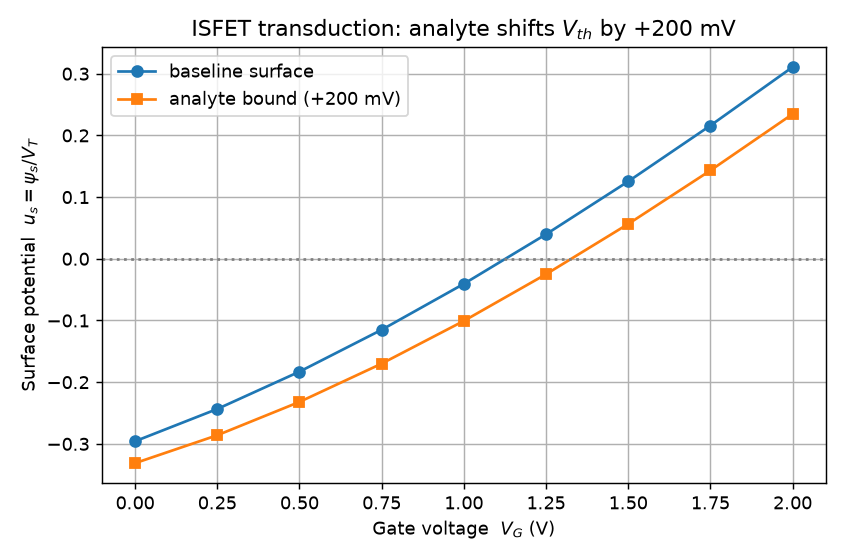
\includegraphics[width=0.72\textwidth]{figures/isfet_moscap.png}
\caption{MOS-capacitor front-end (\code{biosensor\_isfet.py}): analyte binding,
modelled as a gate work-function step, rigidly shifts the surface-potential
characteristic --- the ISFET transduction principle.}
\label{fig:moscap}
\end{figure}

\subsection{Full-device transfer curves}
Figure~\ref{fig:transfer} shows the $I_D(V_G)$ transfer curves (linear and
semilog) for a series of analyte steps. Table~\ref{tab:transfer} lists the
extracted figures of merit. The coupling is exactly unity
($dV_{\mathrm{th}}/d\Phi=1.000$), the ideal limit, because the bare device has
no electrolyte; the sub-threshold swing $S\approx135$~mV/dec exceeds the 60
mV/dec thermal limit, reflecting the short-channel geometry.

\begin{figure}[htbp]
\centering
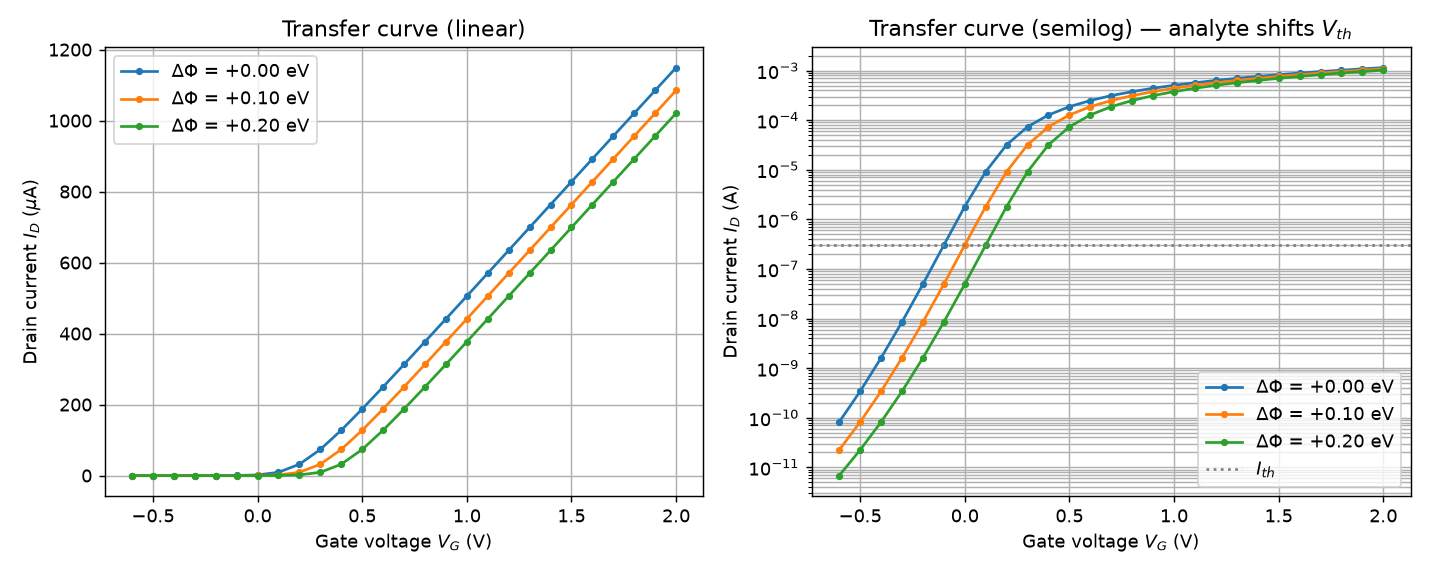
\includegraphics[width=\textwidth]{figures/isfet_transfer.png}
\caption{Full ISFET transfer curves (\code{biosensor\_isfet\_transfer.py}):
analyte-induced work-function steps translate the $I_D(V_G)$ characteristic; the
threshold shift is the sensor signal.}
\label{fig:transfer}
\end{figure}

\begin{table}[htbp]
\centering
\caption{Transfer-curve figures of merit ($W=1~\mu$m, $V_D=0.1$~V).}
\label{tab:transfer}
\begin{tabular}{@{}rrrrr@{}}
\toprule
$\Delta\Phi$ (eV) & $V_{\mathrm{th}}$ (V) & $\Delta V_{\mathrm{th}}$ (mV) & $S$ (mV/dec) & $I_{\mathrm{on}}$ (A) \\
\midrule
$+0.00$ & $-0.099$ & 0   & 135 & $1.15\ee{-3}$ \\
$+0.10$ & $+0.001$ & 100 & 135 & $1.09\ee{-3}$ \\
$+0.20$ & $+0.101$ & 200 & 135 & $1.02\ee{-3}$ \\
\midrule
\multicolumn{5}{@{}l}{Sensitivity $dV_{\mathrm{th}}/d\Phi = 1.000$~V/V (ideal, unity coupling).} \\
\bottomrule
\end{tabular}
\end{table}

\subsection{Electrolyte double layer and the realistic biosensor}
Figure~\ref{fig:gdl} shows the site-binding surface-potential response (left,
its slope is the sub-Nernstian sensitivity) and the Debye-screening collapse of
bound-charge detection with ionic strength (right). Table~\ref{tab:gdl}
summarises the sub-Nernstian pH sensitivity for four representative oxides, and
Table~\ref{tab:debye} the screening collapse. When the electrolyte module drives
the full device solve (\code{--device}), the transistor threshold sensitivity is
electrolyte-limited: $dV_{\mathrm{th}}/d\mathrm{pH}=57.4$~mV/pH for Ta$_2$O$_5$
and $24.6$~mV/pH for SiO$_2$ --- both below the 59.5~mV/pH Nernst limit, unlike
the ideal-coupling models.

\begin{figure}[htbp]
\centering
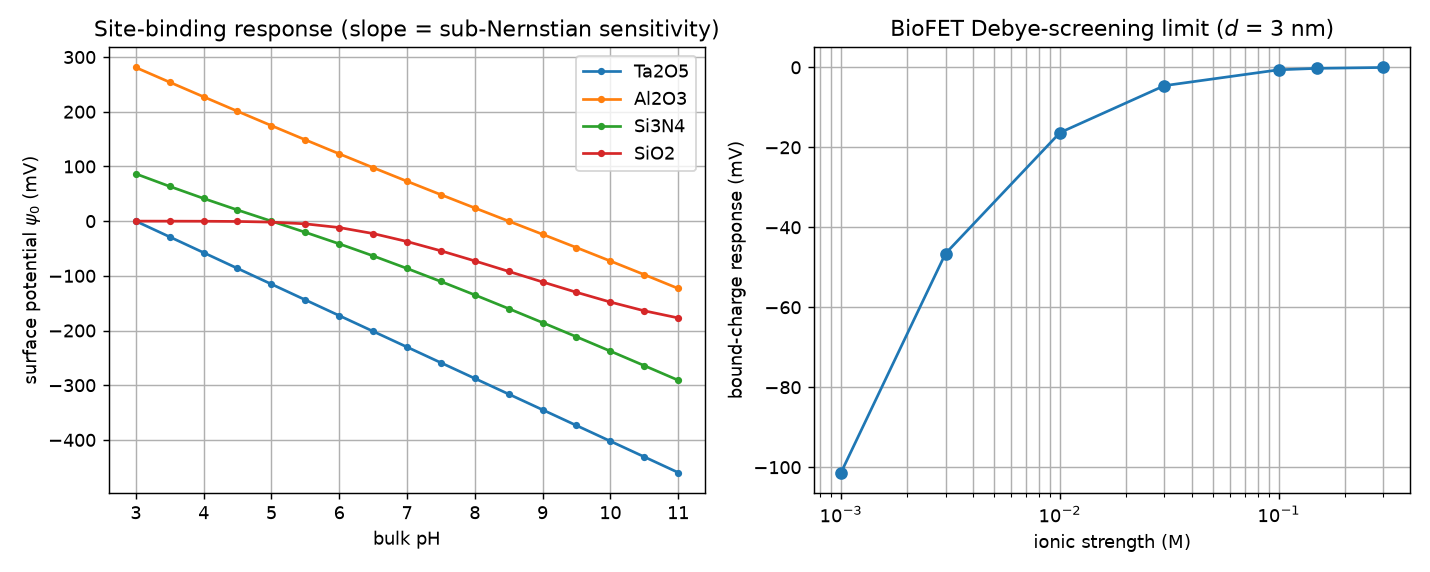
\includegraphics[width=\textwidth]{figures/isfet_gdl.png}
\caption{Electrolyte double-layer model (\code{double\_layer.py} /
\code{biosensor\_isfet\_gdl.py}). Left: site-binding surface potential
$\psi_0(\mathrm{pH})$ --- the slope is the sub-Nernstian sensitivity. Right: the
Debye-screening limit --- a bound charge at $d=3$~nm becomes undetectable as the
ionic strength shrinks $\lambda_D$ below $d$.}
\label{fig:gdl}
\end{figure}

\begin{table}[htbp]
\centering
\begin{minipage}[t]{0.48\textwidth}
\centering
\caption{Sub-Nernstian pH sensitivity at pH~7, $I=0.15$~M (Nernst limit
59.2~mV/pH).}
\label{tab:gdl}
\begin{tabular}{@{}lrr@{}}
\toprule
oxide & mV/pH & $\alpha$ \\
\midrule
Ta$_2$O$_5$ & 57.4 & 0.97 \\
Al$_2$O$_3$ & 49.5 & 0.84 \\
Si$_3$N$_4$ & 46.9 & 0.79 \\
SiO$_2$     & 31.6 & 0.53 \\
\bottomrule
\end{tabular}
\end{minipage}\hfill
\begin{minipage}[t]{0.48\textwidth}
\centering
\caption{BioFET Debye screening: bound charge $-0.01$~C/m$^2$ at $d=3$~nm.}
\label{tab:debye}
\begin{tabular}{@{}rrr@{}}
\toprule
$I$ (M) & $\lambda_D$ (nm) & response (mV) \\
\midrule
0.001 & 9.62 & $-101.3$ \\
0.010 & 3.04 & $-16.3$ \\
0.100 & 0.96 & $-0.61$ \\
0.150 & 0.79 & $-0.25$ \\
\bottomrule
\end{tabular}
\end{minipage}
\end{table}

% =========================================================================
\section{Applications to disease detection}
\label{sec:apps}

The models map directly onto label-free diagnostic devices. In each case the
analyte alters the interfacial surface potential $\psi_0$, which shifts the
threshold via Eq.~\eqref{eq:map}:
\begin{itemize}
  \item \textbf{pH / metabolic panels} --- direct proton response
  (Eq.~\eqref{eq:alpha}); oxide choice sets the sensitivity.
  \item \textbf{DNA-FET} --- hybridisation adds phosphate-backbone charge; the
  Debye limit (Eq.~\eqref{eq:debye}) dictates that low ionic strength or short
  probes are required.
  \item \textbf{ImmunoFET} --- antigen--antibody binding charge; troponin/CRP
  cardiac and inflammatory markers.
  \item \textbf{Enzymatic (glucose) FET} --- enzyme reaction changes local pH,
  read out as in the pH case.
  \item \textbf{Wide-bandgap / nanowire variants} --- SiC/GaN surfaces for
  harsh-media and implantable sensing; thin-body nanowire BioFETs where the
  DDM.SPC Schr\"odinger--Poisson correction captures the confinement-enhanced
  sensitivity.
\end{itemize}

% =========================================================================
\section{Limitations and outlook}
\label{sec:limits}

The device solver is steady-state (no transient/AC, so binding kinetics and
low-frequency noise are out of scope) and has no photogeneration or self-heating.
The electrolyte module uses a mean-field 2-pK site-binding + Gouy--Chapman--Stern
description; the per-oxide $(N_s,\mathrm{p}K_a,\mathrm{p}K_b)$ parameters are
illustrative values chosen to reproduce the known ISFET ordering and sensitivity
ranges and should be re-fit to a given fabrication. Natural extensions are a
transient continuity solve for kinetics/impedance and a quantum-corrected
nanowire BioFET that exploits the solver's confinement model for enhanced
sensitivity.

% =========================================================================
\begin{thebibliography}{9}
\small
\bibitem{bergveld1970} P.~Bergveld, ``Development of an ion-sensitive solid-state
device for neurophysiological measurements,'' \emph{IEEE Trans. Biomed. Eng.},
vol.~BME-17, pp.~70--71, 1970.
\bibitem{bergveld2003} P.~Bergveld, ``Thirty years of ISFETOLOGY,''
\emph{Sensors and Actuators B}, vol.~88, pp.~1--20, 2003.
\bibitem{yates1974} D.~E.~Yates, S.~Levine, T.~W.~Healy, ``Site-binding model of
the electrical double layer at the oxide/water interface,'' \emph{J. Chem. Soc.
Faraday Trans. 1}, vol.~70, pp.~1807--1818, 1974.
\bibitem{fung1986} C.~D.~Fung, P.~W.~Cheung, W.~H.~Ko, ``A generalized theory of
an electrolyte-insulator-semiconductor field-effect transistor,'' \emph{IEEE
Trans. Electron Devices}, vol.~33, pp.~8--18, 1986.
\bibitem{vanhal1996} R.~E.~G.~van Hal, J.~C.~T.~Eijkel, P.~Bergveld, ``A general
model to describe the electrostatic potential at electrolyte oxide interfaces,''
\emph{Adv. Colloid Interface Sci.}, vol.~69, pp.~31--62, 1996.
\bibitem{poghossian2014} A.~Poghossian, M.~J.~Sch\"oning, ``Label-free sensing of
biomolecules with field-effect devices,'' \emph{Electroanalysis}, vol.~26,
pp.~1197--1213, 2014.
\bibitem{schoning2002} M.~J.~Sch\"oning, A.~Poghossian, ``Recent advances in
biologically sensitive field-effect transistors (BioFETs),'' \emph{Analyst},
vol.~127, pp.~1137--1151, 2002.
\bibitem{sze} S.~M.~Sze, K.~K.~Ng, \emph{Physics of Semiconductor Devices}, 3rd
ed., Wiley, 2007.
\bibitem{selberherr} S.~Selberherr, \emph{Analysis and Simulation of
Semiconductor Devices}, Springer, 1984.
\bibitem{nair2007} P.~R.~Nair, M.~A.~Alam, ``Design considerations of silicon
nanowire biosensors,'' \emph{IEEE Trans. Electron Devices}, vol.~54,
pp.~3400--3408, 2007.
\bibitem{stern1972} F.~Stern, ``Self-consistent results for $n$-type Si inversion
layers,'' \emph{Phys. Rev. B}, vol.~5, pp.~4891--4899, 1972.
\end{thebibliography}

\end{document}
